\documentclass[12pt]{amsart}
\usepackage{enumerate}
\usepackage[colorlinks=true, linkcolor=blue, urlcolor=blue, citecolor=blue, anchorcolor=blue, pdfborder={0 0 0}]{hyperref}
\usepackage{url}
\usepackage{graphicx,color}
\usepackage{cite}
\usepackage{amsthm, amsmath, amssymb}
\usepackage{mathtools}
\usepackage[top=45truemm, bottom=45truemm, left=30truemm, right=30truemm]{geometry}
\usepackage{nicefrac}
\usepackage{cancel}
\usepackage{float}
\usepackage{tabularx}
\usepackage{makecell}
\usepackage{array}
\usepackage{ragged2e}

\newcolumntype{P}[1]{>{\RaggedRight\hspace{0pt}}p{#1}}

\newcolumntype{L}{>{\begin{math}}l<{\end{math}}}%
\newcolumntype{C}{>{\begin{math}}c<{\end{math}}}%
\newcolumntype{R}{>{\begin{math}}r<{\end{math}}}%

\newtheorem{theorem}{Theorem}
\newtheorem{lemma}{Lemma}
\newtheorem{corollary}{Corollary}
\newtheorem{definition}{Definition}
\newtheorem{proposition}{Proposition}
\newtheorem{example}{Example}
\theoremstyle{definition}
\newtheorem{remark}{Remark}

\DeclareMathOperator{\len}{len}

\setlength{\headsep}{2em}
\setlength{\skip\footins}{1.4pc plus 5pt minus 2pt}

\title[Rational Points in Elliptic Curves]{Rational Points in Elliptic Curves \boldmath$y^2=x^3-pqx$}

\author[E.\ Sultanow]{\href{https://orcid.org/0000-0001-5257-2236}{
\includegraphics[scale=0.06]{orcid.png}}\hspace{1mm}Eldar Sultanow}
\address{Eldar Sultanow\\Capgemini\\Bahnhofstraße 30\\90402 Nuremberg\\Germany}
\curraddr{}
\email{eldar.sultanow@capgemini.com}

\author[M.\ Amir]{Malik Amir}
\address{Malik Amir\\École Polytechnique Fédérale de Lausanne\\CH-1015 Lausanne\\Switzerland}
\curraddr{}
\email{malik.amir@epfl.ch}

\author[S.\ Ghosh]{Sourangshu Ghosh}
\address{Sourangshu Ghosh\\Indian institute of Technology Kharagpur\\Kharagpur, West Bengal 721302\\India}
\curraddr{}
\email{sourangshu@iitkgp.ac.in}

\author[J.\ Jormakka]{Jorma Jormakka}
\address{Jorma Jormakka\\Aalto University\\Department of Communications and Networking\\Helsinki\\Finland}
\curraddr{}
\email{jorma.o.jormakka@gmail.com}

\subjclass[2010]{14H52}
\keywords{Elliptic Curves, Rational Points}

\begin{document}
	
	\begingroup
	\let\MakeUppercase\relax
	\maketitle
	\endgroup
	
	\begin{abstract}
		Let $p$ and $q$ be two distinct primes and $p\le q$. This paper distills the conditions that both primes must satisfy in order for the elliptic curve $y^2=x^3-pqx$ to have rational solutions. These conditions establish the basis for proving that any elliptic curve of this form has a rational solution.
	\end{abstract}
	
	\section{Introduction}
	\label{introduction}
	The fact whether an elliptic curve has rational points or not has been occupying mathematicians for a fairly while. There are stringent conditions under which elliptic curves have definitely rational points. We lay the foundation for a weaker condition under which elliptic curves are guaranteed to feature rational points.
	
	\section{\texorpdfstring{Conditions for the curve $y^2=x^3-pqx$ to have a rational solution}{Conditions for the curve y2=x3-pqx to have a rational solution}}
	\label{conditions}
	
	We intersect a linear function $y=\nicefrac{a}{b}\cdot x$ that has a rational slope ($a,b\in\mathbb{Z}$) with the elliptic curve $y^2=x^3-pqx$. In order to retrieve the intersection points we must solve the following equation~\ref{eq:solve_rational_points}:
	
	\begin{equation}
		\label{eq:solve_rational_points}
		0=x^3-\left(\frac{a}{b}\right)^2x^2-pqx
	\end{equation}
	
	One intersection point trivially is $(x,y)=(0,0)$. The two remaining intersection points we retrieve by the quadratic formula~\ref{eq:quadratic_formula}:
	
	\begin{equation}
		\label{eq:quadratic_formula}
		x=\frac{1}{2}\left(\frac{a}{b}\right)^2\pm\sqrt{\frac{\left(\frac{a}{b}\right)^4+4pq}{4}}
	\end{equation}
	
	We can slightly convert the discriminant (the term under the square root) such that one can recognize at a glimpse the condition to be met for obtaining a rational solution:
	
	\begin{equation}
		\label{eq:discriminant}
		\Delta=\frac{a^4+4pqb^4}{4b^4}
	\end{equation}
	
	In order to obtain a rational solution, the sum $a^4+4pqb^4=c^2$ must be a square number. We get $4pqb^4=c^2-a^4=(c-a^2)(c+a^2)$. Now there exist several cases to be considered, how the factors $2\cdot2\cdot p\cdot q\cdot b\cdot b\cdot b\cdot b$ are assigned to the two factors $(c-a^2)$ and $(c+a^2)$.
	
	One case is $c-a^2=2pq$ and $c+a^2=2b^4$ which after substracting both equations from each other leads to $2pq=2b^4-2a^2$ providing the condition that $pq$ must be a difference of a fourth power and square number $pq=b^4-a^2$. This case has number $26$ and it is listed in the 26th row of Table~\ref{table:cases_inv}. Let us retrace this principle by an example $p=3$ and $q=5$. In this case $3\cdot5=2^4-1^2=b^4-a^2$ and thus $c=31$ and the discriminant $\Delta=\nicefrac{961}{64}$ which finally leads to the rational solutions $(x,y)=(4,2)$ and $(x,y)=(\nicefrac{-15}{4},\nicefrac{-15}{8})$. This curve is listed in the LMFDB \cite{LMFDB_14400.cq1} too.
	
	Finding all possibilities to split the set $P=\{2,2,p,q,b,b,b,b\}$ of elements (factors) into two subsets is equivalent to finding half the number of divisors of $2^2pqb^4$. For this we can use the divisor function $\tau(n)$, also denoted as $d(n)$ or $\sigma_0(n)$, which returns the number of positive divisors of $n$, see \cite[p.~123]{Fine_Rosenberger_2007}, \cite{OEIS_A000005}. Suppose that $n=p_1^{e_1}\cdots p_k^{e_k}$, then we obtain the number of divisors via $\tau(n)=(e_1+1)\cdots(e_k+1)$, see \cite[p.~125]{Fine_Rosenberger_2007}.
	
	In our case the number of possibilities for splitting the set $P$ into two subsets is:
	
	\[
	\frac{1}{2}\tau(2^2pqb^4)=\frac{1}{2}(2+1)(1+1)(1+1)(4+1)=30
	\]
	
	\par\medskip
	The corresponding combinations (numbered cases) are:
	
	\[
	{\renewcommand{\arraystretch}{1.2}
		\begin{array}{rlrlrlrl}
			1&(22pqbbbb,\emptyset)&9&(22qbbbb,p)&16&(22pbbbb,q)&23&(2b,2pqbbb)\\
			2&(2pqbbbb,2)&10&(2qbbbb,p2)&17&(2pbbbb,q2)&24&(2bb,2pqbb)\\
			3&(pqbbbb,22)&11&(qbbbb,p22)&18&(pbbbb,q22)&25&(2bbb,2pqb)\\
			4&(bbbb,22pq)&12&(qbbb,p22b)&19&(pbbb,q22b)&26&(2bbbb,2pq)\\
			5&(bbb,22pqb)&13&(qbb,p22bb)&20&(pbb,q22bb)&27&(22b,pqbbb)\\
			6&(bb,22pqbb)&14&(qb,p22bbb)&21&(pb,q22bbb)&28&(22bb,pqbb)\\
			7&(b,22pqbbb)&15&(q,p22bbbb)&22&(p,q22bbbb)&29&(22bbb,pqb)\\
			8&(\emptyset,22pqbbbb)&&&&&30&(22bbbb,pq)
	\end{array}}
	\]
	
	\par\medskip
	At this point we accept that (because $b$ is not necessarily prime) not all cases are covered. Table~\ref{table:cases} and \ref{table:cases_inv} deduce from these cases the conditions that both primes $p,q$ must satify for the curve $y^2=x^3-pqx$ to have a rational solution.
	
	In some cases the conditions overlap, for example condition 19 in Table~\ref{table:cases_inv} leads directly to condition 25 when substituting $a$ with $\nicefrac{2a}{p}$ and $b$ with $\nicefrac{2b}{p}$:
	
	\[
	q=\frac{p\left(\frac{2b}{p}\right)^3-2\left(\frac{2a}{p}\right)^2}{4\frac{2b}{p}}=\frac{p(8pb^3-8pa^2)}{8p^3b}=\frac{b^3-a^2}{pb}
	\]
	
	\par\medskip
	Similarly, condition 12 in Table~\ref{table:cases_inv} leads to condition 25 when $a$ is replaced with $\nicefrac{2a}{q}$ and $b$ with $\nicefrac{2b}{q}$.
	
	In Table~\ref{table:cases_inv}, substituting $a$ with $2a$ and $b$ with $2b$ leads condition in case 3 to the condition given by case 1, and similarly case 4 leads to case 30, case 11 leads to case 9, and case 18 to case 16. The same occurs with the equal-numbered cases in Table~\ref{table:cases}.
	
	In Table~\ref{table:cases}, case 1 is identical to case 8 in Table~\ref{table:cases_inv} and, conversely, case 8 in Table~\ref{table:cases} is identical to case 1 in Table~\ref{table:cases_inv}.
	
	In Table~\ref{table:cases}, replacing $b$ with $-b$ brings the conditions of cases 5,7,12,14,19,21,23,25,27,29 to the same-numbered cases in Table~\ref{table:cases_inv}.
	
	Moreover condition 1 in Table~\ref{table:cases} (which is equal to condition 8 in Table~\ref{table:cases_inv}) is impossible, since $4b^4pq+2a^2=1$ has no integer solutions $a,b$. For the same reason, the condition given by case 2 in Table~\ref{table:cases} can never be satisfied too.
	
	\newpage
	{\renewcommand{\arraystretch}{1.2}
		\begin{table}[H]
			\centering
			\begin{tabular}{|l|l|l|l|l|l|l|l|}
				\hline
				\thead[l]{\textbf{Case}} &
				\thead[l]{$\boldsymbol{c-a^2}$} &
				\thead[l]{$\boldsymbol{c+a^2}$} &
				\thead[l]{\textbf{Condition}} &
				\thead[l]{\textbf{Sample Curve}} &
				\thead[l]{$\boldsymbol{a,b,c}$} &
				\thead[l]{$\boldsymbol{\Delta}$} &
				\thead[l]{\textbf{Rational Points}}
				\\
				\hline
				1 &
				$4pqb^4$ &
				$1$ &
				$pq=\nicefrac{1-2a^2}{4b^4}$ &
				Tab.~\ref{table:cases_inv}, case 8 &
				&
				&
				
				\\
				\hline
				2 &
				$2pqb^4$ &
				$2$ &
				$pq=\nicefrac{1-a^2}{b^4}$ &
				impossible &
				&
				&
				
				\\
				\hline
				3 &
				$pqb^4$ &
				$4$ &
				$pq=\nicefrac{4-2a^2}{b^4}$ &
				see case 1 &
				&
				&
				
				\\
				\hline
				4 &
				$b^4$ &
				$4pq$ &
				$pq=\nicefrac{2a^2+b^4}{4}$ &
				see case 30 &
				&
				&
				
				\\
				\hline
				5 &
				$b^3$ &
				$4pqb$ &
				$pq=\nicefrac{2a^2+b^3}{4b}$ &
				Tab.~\ref{table:cases_inv}, case 5 &
				&
				&
				
				\\
				\hline
				6 &
				$b^2$ &
				$4pqb^2$ &
				$pq=\nicefrac{2a^2+b^2}{4b^2}$ &
				&
				&
				&
				
				\\
				\hline
				7 &
				$b$ &
				$4pqb^3$ &
				$pq=\nicefrac{2a^2+b}{4b^3}$ &
				Tab.~\ref{table:cases_inv}, case 7 &
				&
				&
				
				\\
				\hline
				8 &
				$1$ &
				$4pqb^4$ &
				$pq=\nicefrac{2a^2+1}{4b^4}$ &
				Tab.~\ref{table:cases_inv}, case 1 &
				&
				&
				
				\\
				\hline
				9 &
				$4qb^4$ &
				$p$ &
				$p=2a^2+4qb^4$ &
				&
				&
				&
				
				\\
				\hline
				10 &
				$2qb^4$ &
				$2p$ &
				$p=a^2+qb^4$ &
				&
				&
				&
				
				\\
				\hline
				11 &
				$qb^4$ &
				$4p$ &
				$p=\nicefrac{2a^2+qb^4}{4}$ &
				see case 9&
				&
				&
				
				\\
				\hline
				12 &
				$qb^3$ &
				$4pb$ &
				$p=\nicefrac{2a^2+qb^3}{4b}$ &
				Tab.~\ref{table:cases_inv}, case 12 &
				&
				&
				
				\\
				\hline
				13 &
				$qb^2$ &
				$4pb^2$ &
				$p=\nicefrac{2a^2+qb^2}{4b^2}$ &
				&
				&
				&
				
				\\
				\hline
				14 &
				$qb$ &
				$4pb^3$ &
				$p=\nicefrac{2a^2+qb}{4b^3}$ &
				Tab.~\ref{table:cases_inv}, case 14 &
				&
				&
				
				\\
				\hline
				15 &
				$q$ &
				$4pb^4$ &
				$p=\nicefrac{2a^2+q}{4b^4}$ &
				&
				&
				&
				
				\\
				\hline
				16 &
				$4pb^4$ &
				$q$ &
				$q=2a^2+4pb^4$ &
				&
				&
				&
				
				\\
				\hline
				17 &
				$2pb^4$ &
				$2q$ &
				$q=a^2+pb^4$ &
				&
				&
				&
				
				\\
				\hline
				18 &
				$pb^4$ &
				$4q$ &
				$q=\nicefrac{2a^2+pb^4}{4}$ &
				see case 16 &
				&
				&
				
				\\
				\hline
				19 &
				$pb^3$ &
				$4qb$ &
				$q=\nicefrac{2a^2+pb^3}{4b}$ &
				Tab.~\ref{table:cases_inv}, case 19 &
				&
				&
				
				\\
				\hline
				20 &
				$pb^2$ &
				$4qb^2$ &
				$q=\nicefrac{2a^2+pb^2}{4b^2}$ &
				&
				&
				&
				
				\\
				\hline
				21 &
				$pb$ &
				$4qb^3$ &
				$q=\nicefrac{2a^2+pb}{4b^3}$ &
				Tab.~\ref{table:cases_inv}, case 21 &
				&
				&
				
				\\
				\hline
				22 &
				$p$ &
				$4qb^4$ &
				$q=\nicefrac{2a^2+p}{4b^4}$ &
				&
				&
				&
				
				\\
				\hline
				23 &
				$2b$ &
				$2pqb^3$ &
				$pq=\nicefrac{a^2+b}{b^3}$ &
				Tab.~\ref{table:cases_inv}, case 23 &
				&
				&
				
				\\
				\hline
				24 &
				$2b^2$ &
				$2pqb^2$ &
				$pq=\nicefrac{a^2+b^2}{b^2}$ &
				&
				&
				&
				
				\\
				\hline
				25 &
				$2b^3$ &
				$2pqb$ &
				$pq=\nicefrac{a^2+b^3}{b}$ &
				Tab.~\ref{table:cases_inv}, case 25 &
				&
				&
				
				\\
				\hline
				26 &
				$2b^4$ &
				$2pq$ &
				$pq=a^2+b^4$ &
				&
				&
				&
				
				\\
				\hline
				27 &
				$4b$ &
				$pqb^3$ &
				$pq=\nicefrac{2a^2+4b}{b^3}$ &
				Tab.~\ref{table:cases_inv}, case 27 &
				&
				&
				
				\\
				\hline
				28 &
				$4b^2$ &
				$pqb^2$ &
				$pq=\nicefrac{2a^2+4b^2}{b^2}$ &
				&
				&
				&
				
				\\
				\hline
				29 &
				$4b^3$ &
				$pqb$ &
				$pq=\nicefrac{2a^2+4b^3}{b}$ &
				Tab.~\ref{table:cases_inv}, case 29 &
				&
				&
				
				\\
				\hline
				30 &
				$4b^4$ &
				$pq$ &
				$pq=2a^2+4b^4$ &
				&
				&
				&
				
				\\
				\hline
			\end{tabular}
			\caption{Conditions for elliptic curves $y^2=x^3-pqx$ to have rational solutions}
			\label{table:cases}
	\end{table}}
	
	\newpage
	{\renewcommand{\arraystretch}{1.2}
		\begin{table}[H]
			\centering
			\begin{tabular}{|l|l|l|l|l|l|l|l|}
				\hline
				\thead[l]{\textbf{Case}} &
				\thead[l]{$\boldsymbol{c-a^2}$} &
				\thead[l]{$\boldsymbol{c+a^2}$} &
				\thead[l]{\textbf{Condition}} &
				\thead[l]{\textbf{Sample Curve}} &
				\thead[l]{$\boldsymbol{a,b,c}$} &
				\thead[l]{$\boldsymbol{\Delta}$} &
				\thead[l]{\textbf{Rational Points}}
				\\
				\hline
				1 &
				$1$ &
				$4pqb^4$ &
				$pq=\nicefrac{2a^2+1}{4b^4}$ &
				&
				&
				&
				
				\\
				\hline
				2 &
				$2$ &
				$2pqb^4$ &
				$pq=\nicefrac{a^2+1}{b^4}$ &
				&
				&
				&
				
				\\
				\hline
				3 &
				$4$ &
				$pqb^4$ &
				$pq=\nicefrac{2a^2+4}{b^4}$ &
				see case 1 &
				&
				&
				
				\\
				\hline
				4 &
				$4pq$ &
				$b^4$ &
				$pq=\nicefrac{b^4-2a^2}{4}$ &
				see case 30 &
				&
				&
				
				\\
				\hline
				5 &
				$4pqb$ &
				$b^3$ &
				$pq=\nicefrac{b^3-2a^2}{4b}$ &
				&
				&
				&
				
				\\
				\hline
				6 &
				$4pqb^2$ &
				$b^2$ &
				$pq=\nicefrac{b^2-2a^2}{4b^2}$ &
				&
				&
				&
				
				\\
				\hline
				7 &
				$4pqb^3$ &
				$b$ &
				$pq=\nicefrac{b-2a^2}{4b^3}$ &
				&
				&
				&
				
				\\
				\hline
				8 &
				$4pqb^4$ &
				$1$ &
				$pq=\nicefrac{1-2a^2}{4b^4}$ &
				impossible &
				&
				&
				
				\\
				\hline
				9 &
				$p$ &
				$4qb^4$ &
				$p=4qb^4-2a^2$ &
				&
				&
				&
				
				\\
				\hline
				10 &
				$2p$ &
				$2qb^4$ &
				$p=qb^4-a^2$ &
				&
				&
				&
				
				\\
				\hline
				11 &
				$4p$ &
				$qb^4$ &
				$p=\nicefrac{qb^4-2a^2}{4}$ &
				see case 9 &
				&
				&
				
				\\
				\hline
				12 &
				$4pb$ &
				$qb^3$ &
				$p=\nicefrac{qb^3-2a^2}{4b}$ &
				see case 25 &
				&
				&
				
				\\
				\hline
				13 &
				$4pb^2$ &
				$qb^2$ &
				$p=\nicefrac{qb^2-2a^2}{4b^2}$ &
				&
				&
				&
				
				\\
				\hline
				14 &
				$4pb^3$ &
				$qb$ &
				$p=\nicefrac{qb-2a^2}{4b^3}$ &
				&
				&
				&
				
				\\
				\hline
				15 &
				$4pb^4$ &
				$q$ &
				$p=\nicefrac{q-2a^2}{4b^4}$ &
				&
				&
				&
				
				\\
				\hline
				16 &
				$q$ &
				$4pb^4$ &
				$q=4pb^4-2a^2$ &
				&
				&
				&
				
				\\
				\hline
				17 &
				$2q$ &
				$2pb^4$ &
				$q=pb^4-a^2$ &
				&
				&
				&
				
				\\
				\hline
				18 &
				$4q$ &
				$pb^4$ &
				$q=\nicefrac{pb^4-2a^2}{4}$ &
				see case 16 &
				&
				&
				
				\\
				\hline
				19 &
				$4qb$ &
				$pb^3$ &
				$q=\nicefrac{pb^3-2a^2}{4b}$ &
				see case 25 &
				&
				&
				
				\\
				\hline
				20 &
				$4qb^2$ &
				$pb^2$ &
				$q=\nicefrac{pb^2-2a^2}{4b^2}$ &
				&
				&
				&
				
				\\
				\hline
				21 &
				$4qb^3$ &
				$pb$ &
				$q=\nicefrac{pb-2a^2}{4b^3}$ &
				&
				&
				&
				
				\\
				\hline
				22 &
				$4qb^4$ &
				$p$ &
				$q=\nicefrac{p-2a^2}{4b^4}$ &
				&
				&
				&
				
				\\
				\hline
				23 &
				$2pqb^3$ &
				$2b$ &
				$pq=\nicefrac{b-a^2}{b^3}$ &
				&
				&
				&
				
				\\
				\hline
				24 &
				$2pqb^2$ &
				$2b^2$ &
				$pq=\nicefrac{b^2-a^2}{b^2}$ &
				&
				&
				&
				
				\\
				\hline
				25 &
				$2pqb$ &
				$2b^3$ &
				$pq=\nicefrac{b^3-a^2}{b}$ &
				$y^2=x^3-77x$ &
				$6,9,1422$ &
				$\frac{6241}{81}$ &
				$(9,6),(-\frac{77}{9},-\frac{154}{27})$
				\\
				\hline
				26 &
				$2pq$ &
				$2b^4$ &
				$pq=b^4-a^2$ &
				$y^2=x^3-15x$ &
				$1,2,31$&
				$\frac{961}{64}$ &
				$(4,2),(-\frac{15}{4},-\frac{15}{8})$
				\\
				\hline
				27 &
				$pqb^3$ &
				$4b$ &
				$pq=\nicefrac{4b-2a^2}{b^3}$ &
				&
				&
				&
				
				\\
				\hline
				28 &
				$pqb^2$ &
				$4b^2$ &
				$pq=\nicefrac{4b^2-2a^2}{b^2}$ &
				&
				&
				&
				
				\\
				\hline
				29 &
				$pqb$ &
				$4b^3$ &
				$pq=\nicefrac{4b^3-2a^2}{b}$ &
				&
				&
				&
				
				\\
				\hline
				30 &
				$pq$ &
				$4b^4$ &
				$pq=4b^4-2a^2$ &
				&
				&
				&
				
				\\
				\hline
			\end{tabular}
			\caption{Conditions for elliptic curves $y^2=x^3-pqx$ to have rational solutions (reversed cases)}
			\label{table:cases_inv}
	\end{table}}
	
	% trim=left bottom right top
	\begin{figure}[H]
		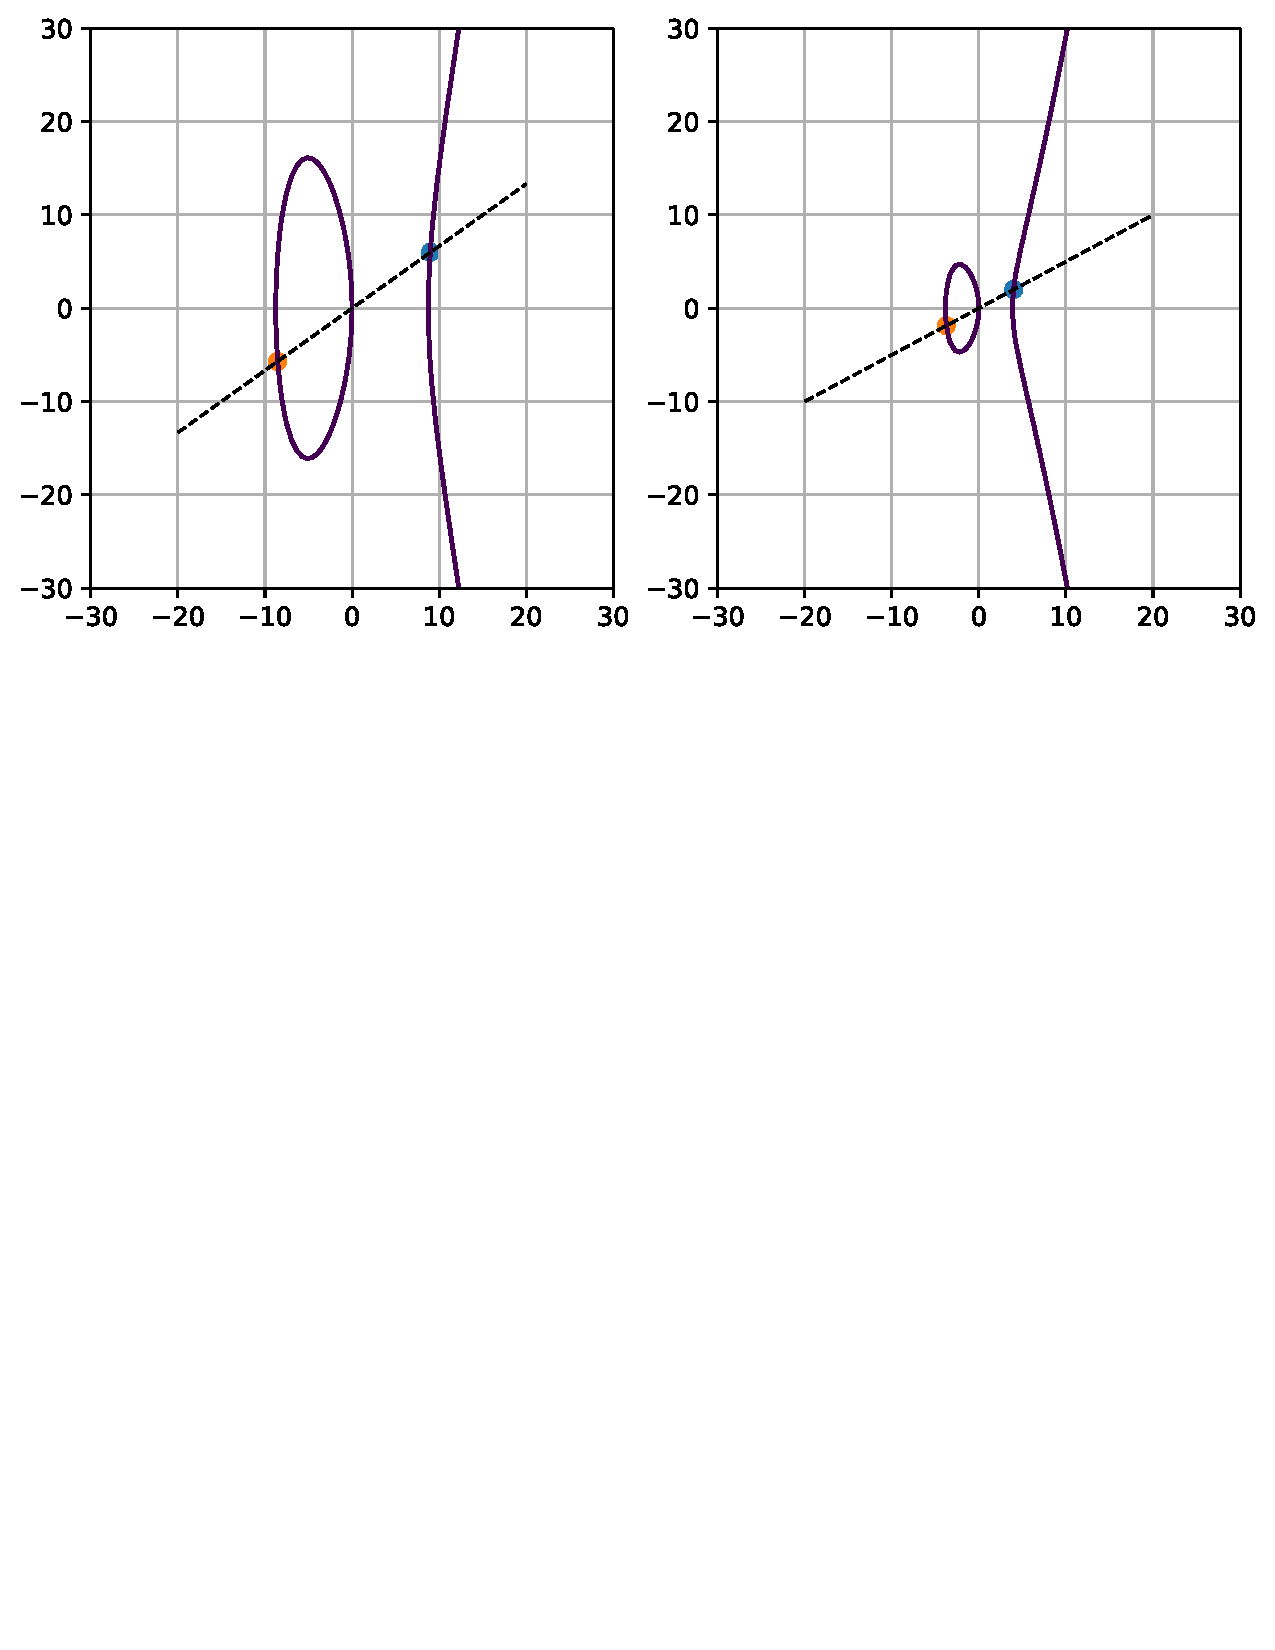
\includegraphics[clip, trim=0cm 17.3cm 0cm 0cm, width=1.00\textwidth, page=1]{figures/curves.pdf}
		\caption{Curves for case 25 (left) and case 26 (right) as given in Table~\ref{table:cases_inv}}
		\label{fig:curves}
	\end{figure}
	
	Figure~\ref{fig:curves} shows the curve $y^2=x^3-77x$ on the left and the curve $y^2=x^3-15x$ on the right as given by the cases 25 and 26 in Table~\ref{table:cases_inv}. The rational points including the intersecting line (that has a slope $\nicefrac{a}{b}$) are depicted too.
	
	\section{Conclusion and Outlook}
	\label{outlook}
	So far, we have inferred the conditions that two distinct odd primes $p,q$ must satisfy for the elliptic curve $y^2=x^3-pqx$ to have rational points. The next step consists in demonstrating that there exist no product of two odd primes $p,q$ for which all these contitions do not match. Inversly stated, at least one of the conditions is true for both primes. That means any product of  two odd primes $p,q$ shall be a congruent number.
	
	%\section{Acknowledgements}
	%\label{acknowledgements}
	%We are grateful for the numerous help from mathematics communities like the \hyperlink{https://math.stackexchange.com}{Stack Exchange Network} or the \hyperlink{https://www.matheboard.de}{MatheBoard Community}. As an example let us mention \hyperlink{https://math.stackexchange.com/users/30382/servaes}{Servaes}, for whose instant help in matters of number theory we are very grateful as for the help by many other kind people from the math communities.
	
	\newpage
	\vspace{1em}
	\bibliographystyle{unsrt}
	\bibliography{main}
\end{document}